\documentclass{sdkslides} 

\usepackage[utf8]{inputenc}
\usepackage[T1]{fontenc}
\usepackage{graphicx}
\usepackage{amssymb,amsmath}
\usepackage{url}
\usepackage{lastpage}
\usepackage{epstopdf}
%\usepackage[pdfpagemode=None,colorlinks=true,urlcolor=red, linkcolor=black,citecolor=black,pdfstartview=FitH]{hyperref}
\usepackage{dirtree}
\usepackage{mdframed}
\usepackage[export]{adjustbox}
\usepackage{caption}
\usepackage{apacite}
\usepackage{tikz}
\usetikzlibrary{positioning,shapes,shadows,arrows}
\tikzset{
  every overlay node/.style={
    %draw=black,fill=white,rounded corners,
    anchor=north west, inner sep=0pt,
  },
  thick/.style=      {line width=0.3mm},
}
\def\tikzoverlay{%
   \tikz[remember picture, overlay]\node[every overlay node]
}%

%%%% This for easy placemnet of figure inside a block
\newcommand{\putfig}[3][1.0]{
    \begin{block}{#3}
        \includegraphics[width=#1\linewidth,height=#1\textheight,keepaspectratio]{#2}
    \end{block}
}
%%%%

%%%% To insert lecture date
%\newcommand{\lectdate}{23.1.2020}
\newcommand{\lectdate}{\today}
%%%%
\newcommand{\sectname}{Section Name}

\title{\Huge{TheSyDeKick}\\ \vspace{0.2in} \normalsize{System development and
verification framework in Python}}

\institute[ELE]{TheSyDeKick Community}

\author{TheSyDeKick contributors}


\sdkfootertext{TheSyDeKick demo}{\lectdate}{\arabic{page}/\pageref{LastPage}\ }

\date{\lectdate}

\newcommand{\tellipse}[4]{
    \begin{tikzpicture}[overlay]
        \draw[secondarycolor,thick] (#1,#2) ellipse (#3 and #4);
    \end{tikzpicture}
}

\newcommand{\tarrow}[2]{
    \begin{tikzpicture}[overlay]
        \draw[secondarycolor,thick,->] (#1) -- (#2);
    \end{tikzpicture}
}

% Copies outline as an sectiontitleslide
%\AtBeginSection[]
%{
%    \begin{frame}{Outline}
%        \tableofcontents[currentsection]
%    \end{frame}
%}
\begin{document}

%%%%%%%%%%%%%%%%%%%%%%%%%%%%%%%%%%%%%%%%%%%%%%%%%%%%%%%%%%%%%%%%%%%%%%%%%%%%%
% Generates the titleframe
\sdktitleframe
%%%%%%%%%%%%%%%%%%%%%%%%%%%%%%%%%%%%%%%%%%%%%%%%%%%%%%%%%%%%%%%%%%%%%%%%%%%%%

%%%%%%%%%%%%%%%%%%%%%%%%%%%%%%%%%%%%%%%%%%
%%%% CONTENTS %%%%%%%%%%%%%%%%%%%%%%%%%%%%
%%%%%%%%%%%%%%%%%%%%%%%%%%%%%%%%%%%%%%%%%%
\section*{Outline}
\begin{frame}[c]
    \frametitle{Outline}
    \tableofcontents
\end{frame}

%%%%%%%%%%%%%%%%%%%%%%%%%%%%%%%%%%%%%%%%%%
%%%% SLIDES BEGIN HERE %%%%%%%%%%%%%%%%%%%
%%%%%%%%%%%%%%%%%%%%%%%%%%%%%%%%%%%%%%%%%%


%%%%%%%%%%%%%%%%%%%%%%%%%%%%%%%%%%%%%%%%%%%%%%%%%%%%%%%%%%%%%%%%%%%%%%%%%%
\sectiontitle[TheSyDeKick - What it is]
\renewcommand{\sectname}{What is it?}
\section{\sectname}
\begin{frame}[t]
    \frametitle{\sectname}
    \centering
        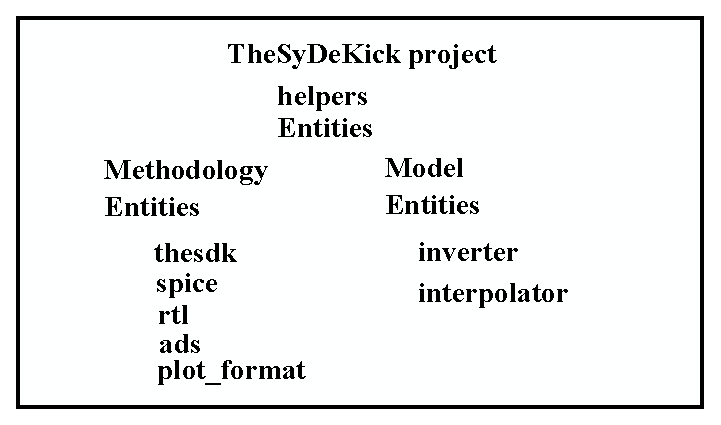
\includegraphics[width=0.3\textwidth]{Pics/TheSyDeKick-entity-principles.eps}
        \begin{itemize}
            \item TheSyDeKick is a well structured container for: 
                \begin{itemize}
                    \item Python packages (Entities), that provide
                        \emph{formalism and methods to run simulations in
                        python, and with external simulators}
                    \item Python packages (Entities), that provide
                        formalism to create and use \emph{IO compatible models}
                \end{itemize}
            \item TheSydeKick is a cumulative collection of Python classes and
                methods that help the designer to carry out the most common
                tasks encountered in microelectronics design. Most likely the
                \emph{simulation task you have in mind has some supporting
                    methodology available in TheSyDeKick}
            \item TheSyDeKick is \emph{nothing more}
        \end{itemize}
\end{frame}

%%%%%%%%%%%%%%%%%%%%%%%%%%%%%%%%%%%%%%%%%%%%%%%%%%%%%%%%%%%%%%%%%%%%%%%%%%%%%
\renewcommand{\sectname}{What is it?}
\begin{frame}[t]
    \frametitle{\sectname}
    \centering
        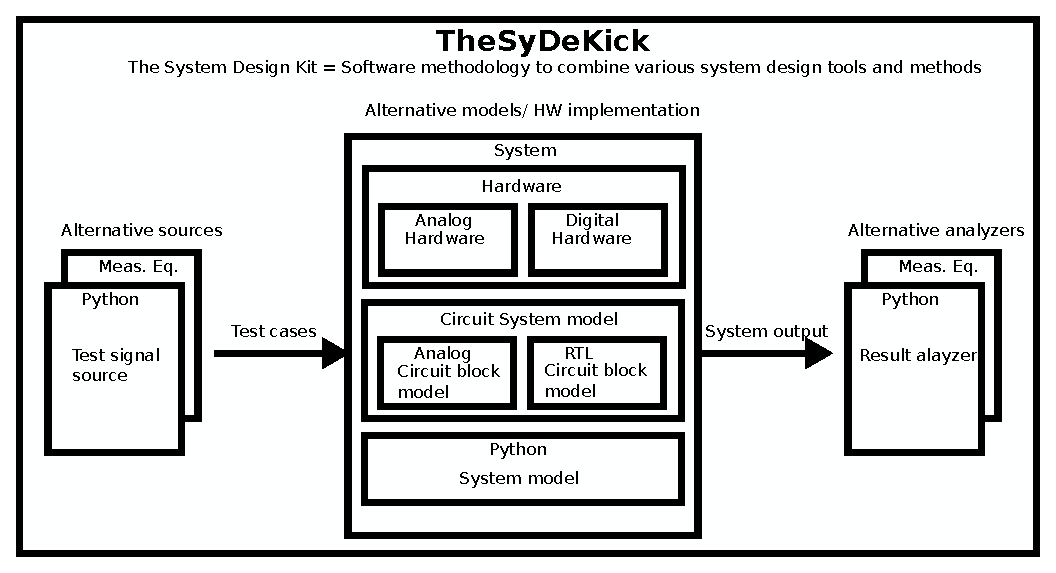
\includegraphics[width=0.65\textwidth]{Pics/TheSDK_block_diagram.eps}
        \begin{itemize}
            \item TheSyDeKick fromalims helps the designed to: 
            \begin{itemize}
                \item Write and simulate modular, hierarchical, IO compatible
                    hardware models wit various levels of abstraction (python,
                    spice/rtl)
                \item Control the abstraction level with one parameter on
                    chosen level of hierarchy.
            \end{itemize}
        \end{itemize}
\end{frame}


%%%%%%%%%%%%%%%%%%%%%%%%%%%%%%%%%%%%%%%%%%%%%%%%%%%%%%%%%%%%%%%%%%%%%%%%%%%%%
\begin{frame}[t]
    \frametitle{\sectname}
    \begin{itemize}
        \item Minimum set of structural constraints, 
            \begin{itemize}
                \item IO definitions
                \item Blocks described as connected \emph{Entities}.
            \end{itemize}
        \item Aims to automation of \emph{repetitive, well structured tasks}
            \begin{itemize}
                \item Model and modeling environment structure with init scripts
                \item Running simulations
                \item Defining simulator calls
                \item Documentation of the design with Docstrings
            \end{itemize}
        \item Currently supports Python, Verilog, VHDL and three spice
            variants.
        \item Under construction: Measurement equipment.
        \item \url{https://github.com/TheSystemDevelopmentKit}
    \end{itemize}
\end{frame}

%%%%%%%%%%%%%%%%%%%%%%%%%%%%%%%%%%%%%%%%%%
\renewcommand{\sectionname}{TheSyDeKick project file structure}
\subsection*{\sectionname}
\begin{frame}[t]
    \frametitle{\sectionname}
    \begin{block}{TheSyDeKick project structure}
    \begin{minipage}[t]{0.3\textwidth}
    \parbox{\textwidth}{
        \dirtree{% 
            .1 thesydekick\_project/.
            .2 Entities/.
            .3 thesdk/.
            .3 rtl/.
            .3 spice/.
            .3 amplifier/.
            .4 amplifier/.
            .5 \_\_init\_\_.py.
            .4 spice/.
            .4 Simulations/.
            .4 doc/.
        }
    }
    \end{minipage}
    \end{block}
\end{frame}


%%%%%%%%%%%%%%%%%%%%%%%%%%%%%%%%%%%%%%%%%%%
%\renewcommand{\sectionname}{ECD BAG project structure}
%\subsection*{\sectionname}
%\begin{frame}[t]
%    \frametitle{\sectionname}
%    \begin{block}{ECD BAG project structure}
%    \begin{minipage}[t]{0.3\textwidth}
%    \parbox{\textwidth}{
%        \dirtree{% 
%            .1 virtuoso\_BAG/.
%            .2 BAG\_technology\_definition/.
%            .2 BAG\_framework/.
%            .2 BAG2\_EC\_TEMPLATES/.
%            .2 bag\_ecd/.
%            .2 amplifier\_bag/.
%            .3 amplifier\_bag/.
%            .4 \_\_init\_\_.py.
%            .4 schematic.py.
%            .4 layout.py.
%            .4 doc/.
%        }
%    }
%    \end{minipage}
%    \end{block}
%\end{frame}
%
%%%%%%%%%%%%%%%%%%%%%%%%%%%%%%%%%%%%%%%%%%%
%\renewcommand{\sectionname}{ECD TheSyDeKick-BAG project structure}
%\subsection*{\sectionname}
%\begin{frame}[t]
%    \frametitle{\sectionname}
%    \begin{block}{TheSyDeKick-BAG project structure}
%    \begin{minipage}[t]{0.41\textwidth}
%    \parbox{\textwidth}{
%        \dirtree{% 
%            .1 thesydekick\_project/.
%            .2 Entities/.
%            .3 thesdk/.
%            .3 spice/.
%            .3 rtl/.
%            .3 amplifier/.
%            .4 amplifier/.
%            .5 \_\_init\_\_.py.
%            .5 schematic.py.
%            .5 layout.py.
%            .4 spice/.
%            .4 Simulations/.
%            .4 doc/.
%        }
%    }
%    \end{minipage}
%    \begin{minipage}[t]{0.41\textwidth}
%    \parbox{\textwidth}{
%        \dirtree{% 
%            .1 virtuoso\_BAG/.
%            .2 BAG\_technology\_definition/.
%            .2 BAG\_framework/.
%            .2 BAG2\_EC\_TEMPLATES/.
%            .2 bag\_ecd/.
%            .2 amplifier/.
%            .3 amplifier/.
%            .4 \_\_init\_\_.py.
%            .4 schematic.py.
%            .4 layout.py.
%            .3 spice/.
%            .3 Simulations/.
%            .3 doc/.
%        }
%    }
%    \end{minipage}
%    \end{block}
%\end{frame}

%%% Additions by Santeri
%%%%%%%%%%%%%%%%%%%%%%%%%%%%%%%%%%%%%%%%%%%%%%%%%%%%%%%%%%%%%%%%%%%%%%%%%%%%%
\sectiontitle[Simulator interfaces]
%%%%%%%%%%%%%%%%%%%%%%%%%%%%%%%%%%%%%%%%%%%%%%%%%%%%%%%%%%%%%%%%%%%%%%%%%%
\renewcommand{\sectname}{Analog simulator interface}
\section{\sectname}
\begin{frame}[t]
    \frametitle{\sectname}
    \begin{itemize}
        \item Calling analog simulators is handled through a common interface, the \textbf{spice} module
        \item Ultimate goal of \textbf{spice}: support for most industry standard simulators
        \begin{itemize}
            \item General (w.r.t to simulator), reusable simulation testbenches
            \item Centralized post processing based on open source tools and
                libraries.
        \end{itemize}
            \item Save time in re-writing testbenches for different simulations and centralize effort to all-in-one testbench
        \begin{itemize}
        \item Currently support for DC, AC, and Transient analysis. Easy to
            add other analysis types as IO formats are the same. 
        \end{itemize}
        \item \url{https://github.com/TheSystemDevelopmentKit/spice}
    \end{itemize}
\end{frame}

%%%%%%%%%%%%%%%%%%%%%%%%%%%%%%%%%%%%%%%%%%%%%%%%%%%%%%%%%%%%%%%%%%%%%%%%%%%%%
\renewcommand{\sectname}{Digital simulator interface}
\section{\sectname}
\begin{frame}[t]
    \frametitle{\sectname}
    \begin{itemize}
        \item Calling digital simulators is handled the \textbf{rtl} module
        %\item \textbf{rtl}: currently supports Questasim
        \begin{itemize}
            \item Most commonly used simulation testbenches automatically
                generated for both Verilog and VHDL design under tests.
            \item Automated file IO generation for strings (bit vectors), integers, and complex numbers. 
            \item Support for any signal type through customizable format
                parameter.
        \end{itemize}
        %\begin{itemize}
        %    \item Future plans: Support for Verilator
        %\end{itemize}
        \item \url{https://github.com/TheSystemDevelopmentKit/rtl}
    \end{itemize}
\end{frame}

%%%%%%%%%%%%%%%%%%%%%%%%%%%%%%%%%%%%%%%%%%%%%%%%%%%%%%%%%%%%%%%%%%%%%%%%%%%%%
\renewcommand{\sectname}{TheSyDeKick simulation procedure}
\begin{frame}[t]
    \frametitle{\sectname}
        \begin{enumerate}
            \item Write the testbench
            \begin{enumerate}
                \item Specify analysis type, inputs, outputs, supplies etc. based on TB properties
                \item Configure simulator options, corners, etc. based on
                    testbench properties
                \item Specify desired outputs, e.g. FFT of waveform, transient waveform
                \item Specify run cases, e.g. transient analysis for 2 different netlists, etc.
            \end{enumerate}
            \item Run the simulation
            \item Analyze results
            \item (Optional) Repeat simulation for different sets of parameters
        \end{enumerate}
        \begin{itemize}
            \item Once you have one testbench, reuse for similar applications makes things faster
            \item Results saved (if user chooses so), no need to repeat lengthy simulations to fix errors in post processing
        \end{itemize}
\end{frame}


%%% End additions by Santeri
%%%%%%%%%%%%%%%%%%%%%%%%%%%%%%%%%%%%%%%%%%%%%%%%%%%%%%%%%%%%%%%%%%%%%%%%%%%%%
\sectiontitle[Design Examples]

%%%%%%%%%%%%%%%%%%%%%%%%%%%%%%%%%%%%%%%%%%%%%%%%%%%%%%%%%%%%%%%%%%%%%%%%%%%%%
\renewcommand{\sectname}{Example 1: Inverter}
\begin{frame}[t]
    \frametitle{\sectname}
    \centering
    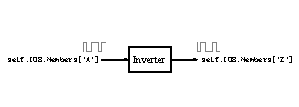
\includegraphics[width=0.95\textwidth]{Pics/inverter_single_1}
    \begin{itemize}
        \item Functional model: Inverts input signal
        \item IOS is a Bundle-type container for storing IO data
        \item Can have as many members as needed
    \end{itemize}
\end{frame}

%%%%%%%%%%%%%%%%%%%%%%%%%%%%%%%%%%%%%%%%%%%%%%%%%%%%%%%%%%%%%%%%%%%%%%%%%%%%%
\begin{frame}[t]
    \frametitle{\sectname}
    \centering
    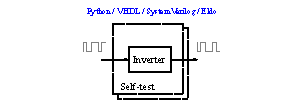
\includegraphics[width=0.95\textwidth]{Pics/inverter_single_2}
    \begin{itemize}
        \item Multiple representations of the same entity
        \item Self-test is a way to verify the functionality of entity ``in
            vacuum''
        \item Self-test generates and feeds the identical input
            data to all simulators
    \end{itemize}
\end{frame}

%%%%%%%%%%%%%%%%%%%%%%%%%%%%%%%%%%%%%%%%%%%%%%%%%%%%%%%%%%%%%%%%%%%%%%%%%%%%%
\renewcommand{\sectname}{Example 2: Inverter Chain}
\section{\sectname}
\begin{frame}[t]
    \frametitle{\sectname}
    \centering
    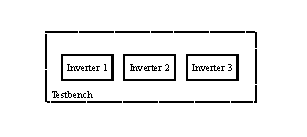
\includegraphics[width=0.95\textwidth]{Pics/inverter_chain_0}
    \begin{itemize}
        \item A separate \textbf{Testbench} entity is instantiated
        \item Chain of inverter instance is created with a for loop
    \end{itemize}
\end{frame}

%%%%%%%%%%%%%%%%%%%%%%%%%%%%%%%%%%%%%%%%%%%%%%%%%%%%%%%%%%%%%%%%%%%%%%%%%%%%%
\begin{frame}[t]
    \frametitle{\sectname}
    \centering
    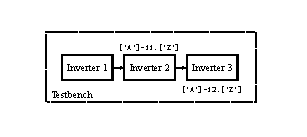
\includegraphics[width=0.95\textwidth]{Pics/inverter_chain_2}
    \begin{itemize}
        \item A separate \textbf{Testbench} entity is instantiated
        \item Chain of inverter instance is created with a for loop
        \item Data flow defined by IOS connections
    \end{itemize}
\end{frame}


%%%%%%%%%%%%%%%%%%%%%%%%%%%%%%%%%%%%%%%%%%%%%%%%%%%%%%%%%%%%%%%%%%%%%%%%%%%%%
\begin{frame}[t]
    \frametitle{\sectname}
    \centering
    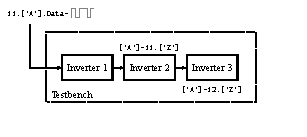
\includegraphics[width=0.95\textwidth]{Pics/inverter_chain_3}
    \begin{itemize}
        \item A separate \textbf{Testbench} entity is instantiated
        \item Chain of inverter instance is created with a for loop
        \item Data flow defined by IOS connections
        \item Testbench input is assigned as input of 1st element
    \end{itemize}
\end{frame}

%%%%%%%%%%%%%%%%%%%%%%%%%%%%%%%%%%%%%%%%%%%%%%%%%%%%%%%%%%%%%%%%%%%%%%%%%%%%%
\begin{frame}[t]
    \frametitle{\sectname}
    \centering
    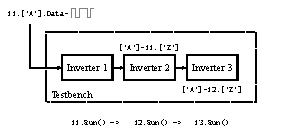
\includegraphics[width=0.95\textwidth]{Pics/inverter_chain_4}
    \begin{itemize}
        \item A separate \textbf{Testbench} entity is instantiated
        \item Chain of inverter instance is created with a for loop
        \item Data flow defined by IOS connections
        \item Testbench input is assigned as input of 1st element
        \item Signal is propagated through the chain by running the entities
            in sequence
    \end{itemize}
\end{frame}

%%%%%%%%%%%%%%%%%%%%%%%%%%%%%%%%%%%%%%%%%%%%%%%%%%%%%%%%%%%%%%%%%%%%%%%%%%%%%
\begin{frame}[t]
    \frametitle{\sectname}
    \centering
    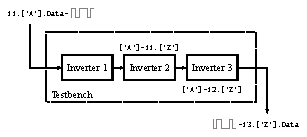
\includegraphics[width=0.95\textwidth]{Pics/inverter_chain_5}
    \begin{itemize}
        \item In the end, the output of the last element contains processed data
    \end{itemize}
\end{frame}

%%%%%%%%%%%%%%%%%%%%%%%%%%%%%%%%%%%%%%%%%%%%%%%%%%%%%%%%%%%%%%%%%%%%%%%%%%%%%
\renewcommand{\sectname}{Example 3: ADC Model}
\section{\sectname} 
\begin{frame}[c]
    \frametitle{\sectname}
    \centering
    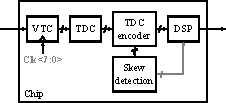
\includegraphics[width=0.9\textwidth]{Pics/sdk_model_0}
\end{frame}
%%%%%%%%%%%%%%%%%%%%%%%%%%%%%%%%%%%%%%%%%%%%%%%%%%%%%%%%%%%%%%%%%%%%%%%%%%%%%
\begin{frame}[c]
    \frametitle{\sectname}
    \centering
    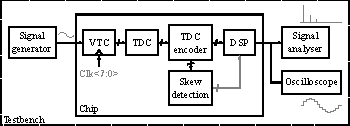
\includegraphics[width=0.9\textwidth]{Pics/sdk_model_1}
\end{frame}

%%%%%%%%%%%%%%%%%%%%%%%%%%%%%%%%%%%%%%%%%%%%%%%%%%%%%%%%%%%%%%%%%%%%%%%%%%%%%
\begin{frame}[c]
    \frametitle{\sectname}
    \centering
    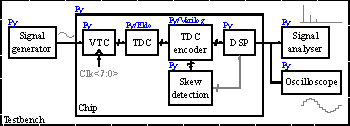
\includegraphics[width=0.9\textwidth]{Pics/sdk_model_2}
\end{frame}

%%%%%%%%%%%%%%%%%%%%%%%%%%%%%%%%%%%%%%%%%%%%%%%%%%%%%%%%%%%%%%%%%%%%%%%%%%%%%
\begin{frame}[c]
    \frametitle{\sectname}
    \centering
    Full ADC Model in Python
    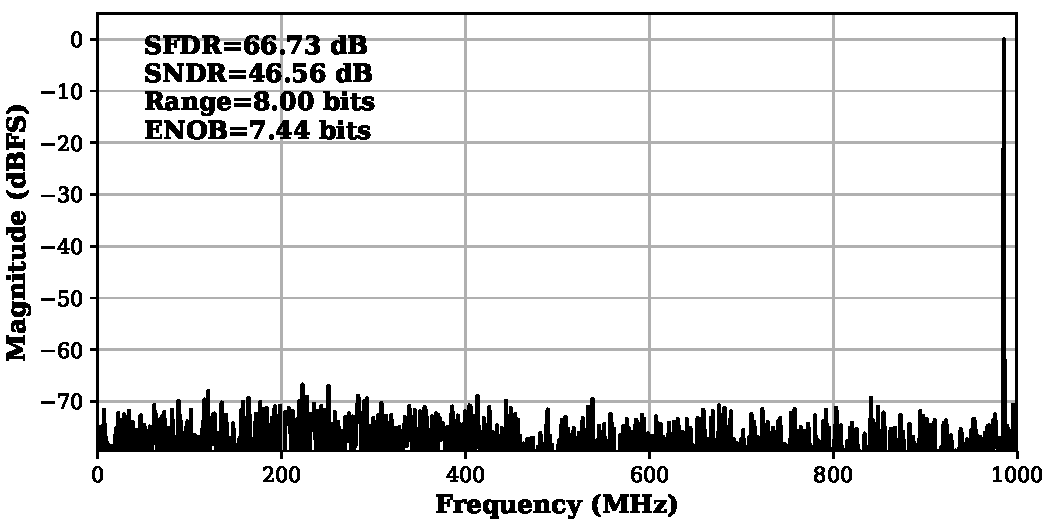
\includegraphics[width=0.8\textwidth]{Pics/latido_fft_py}
    \begin{itemize}
        \item Spectrum plotted by signal\_analyser -module, which also
            calculates SNDR etc.
    \end{itemize}
\end{frame}

%%%%%%%%%%%%%%%%%%%%%%%%%%%%%%%%%%%%%%%%%%%%%%%%%%%%%%%%%%%%%%%%%%%%%%%%%%%%%
\begin{frame}[c]
    \frametitle{\sectname}
    \centering
    Full ADC Model in Python with Transistor-level TDC Model
    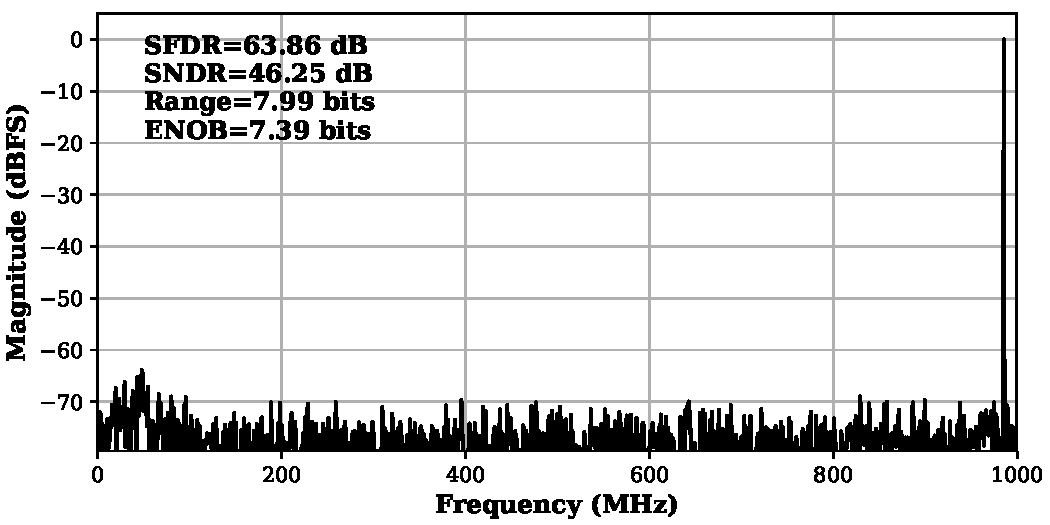
\includegraphics[width=0.8\textwidth]{Pics/latido_fft_eldo}
    \begin{itemize}
        \item Same exact simulation as before, except the TDC block is
            simulated as a spice-netlist in Eldo
    \end{itemize}
\end{frame}

%%%%%%%%%%%%%%%%%%%%%%%%%%%%%%%%%%%%%%%%%%
\renewcommand{\sectionname}{Example 4: Multi-user MIMO receiver}
\subsection*{\sectionname}
\begin{frame}[t]
    \frametitle{\sectionname}
    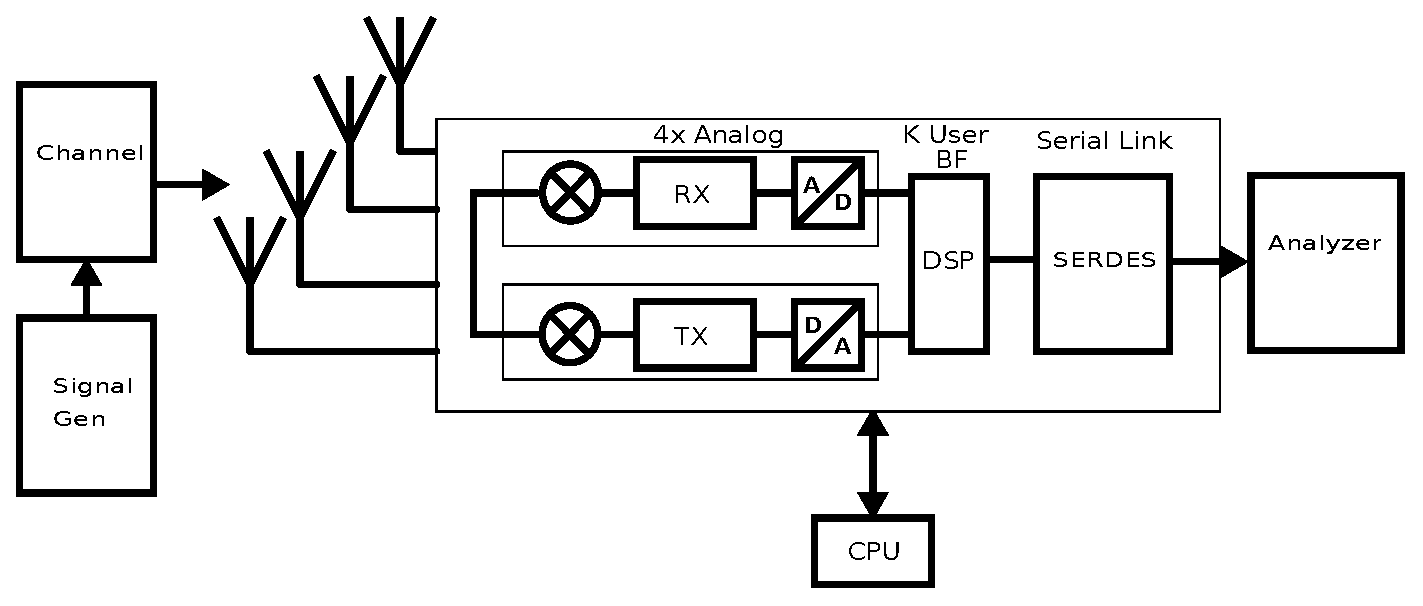
\includegraphics[width=\textwidth]{Pics/Fader2_simulator.eps}
    \begin{itemize}
        \item Goals:
            \begin{itemize}
                \item  First, model the receiver of a single chip with python
                \item  Python models swappable to RTL and analog models 
                \item  Generated sub-blocks verified at the system level
                \item  Control the HW generators of the block (emerging feature)
            \end{itemize}

    \end{itemize}
\end{frame}
%%%%%%%%%%%%%%%%%%%%%%%%%%%%%%%%%%%%%%%%%%
\renewcommand{\sectionname}{DSP modeling example}
\subsection*{\sectionname}
\begin{frame}[c]
    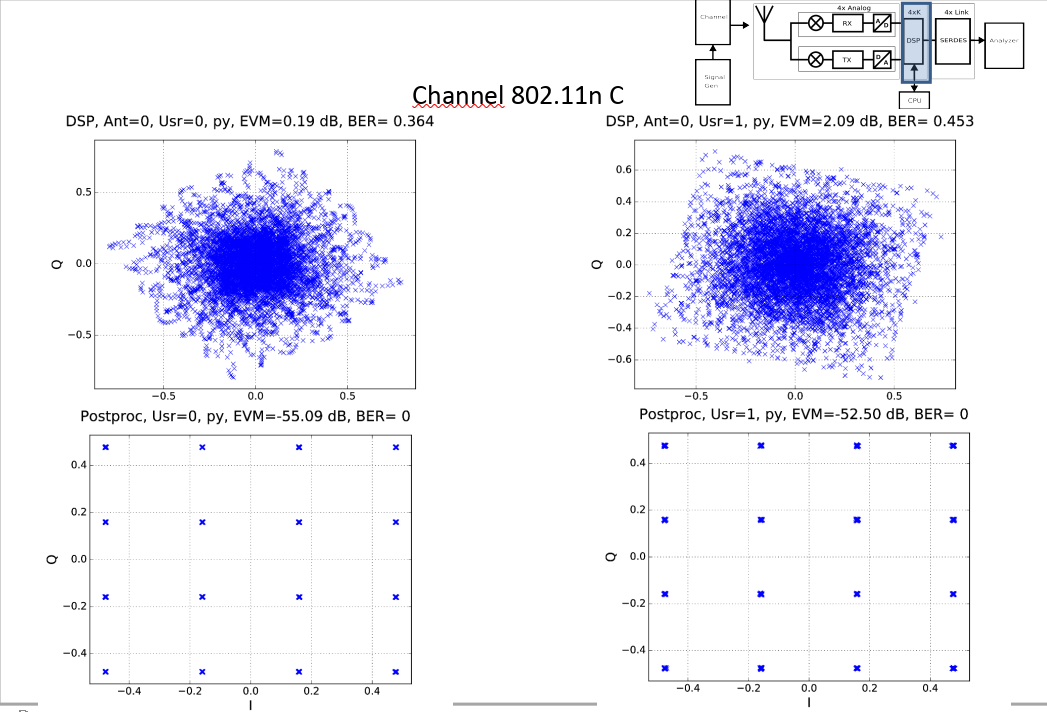
\includegraphics[width=\textwidth]{Pics/DSP-example-fader2-ideal.png}
\end{frame}

%%%%%%%%%%%%%%%%%%%%%%%%%%%%%%%%%%%%%%%%%%
\renewcommand{\sectionname}{Python/RTL example simulation}
\subsection*{\sectionname}
\begin{frame}[c]
    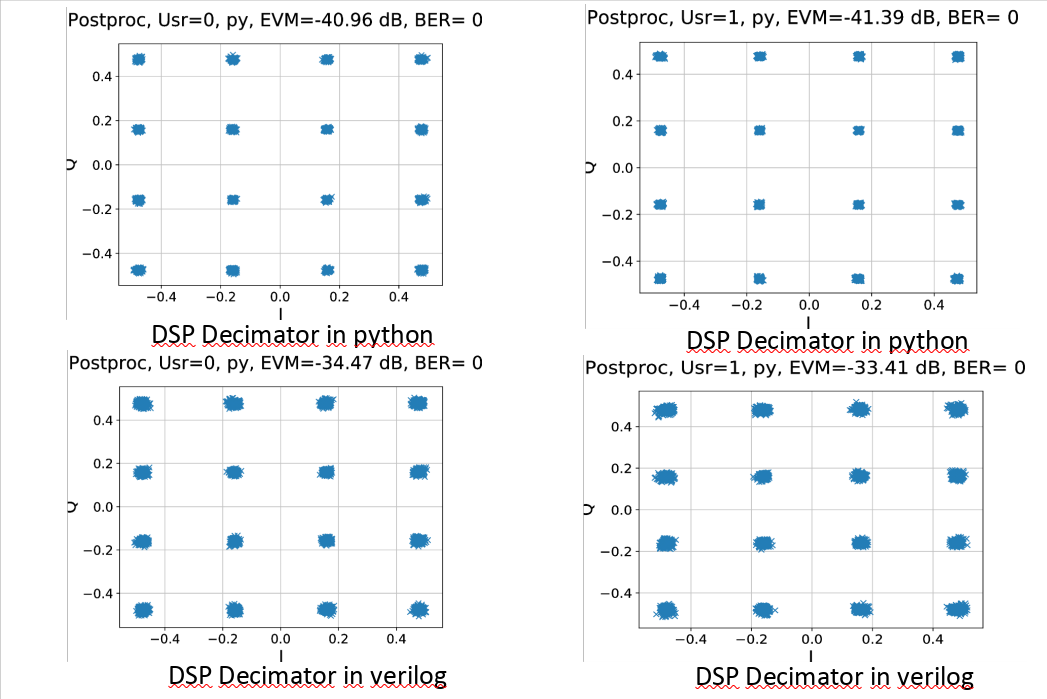
\includegraphics[width=\textwidth]{Pics/DSP-example-fader2-decimator_effect.png}
\end{frame}

%%%%%%%%%%%%%%%%%%%%%%%%%%%%%%%%%%%%%%%%%%
\renewcommand{\sectionname}{Example 5: Outphasing transmitter}
\subsection*{\sectionname}
\begin{frame}[c]
    \frametitle{\sectionname}
    \centering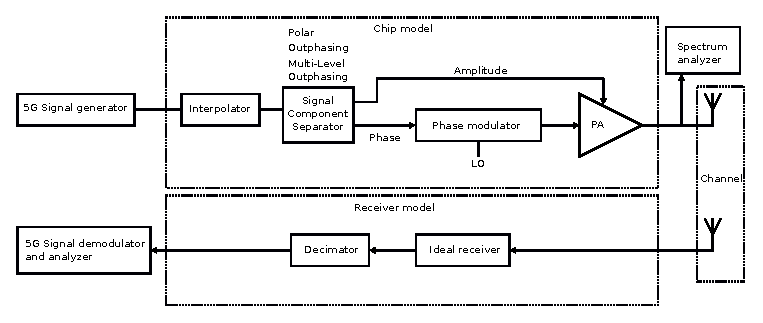
\includegraphics[width=\textwidth]{Pics/HT_system.eps}
    \begin{itemize}
        \item System development
            \begin{itemize}
                \item  Model the transmitter chip with python
                \item  Model the ideal receiver in python
                \item  Simulate the functionality
            \end{itemize}
    \end{itemize}
\end{frame}

%%%%%%%%%%%%%%%%%%%%%%%%%%%%%%%%%%%%%%%%%%
%\subsection*{\sectionname}
\begin{frame}[c]
    \frametitle{\sectionname}
    \includegraphics[width=0.48\textwidth]{Pics/scs_out1+2_20b_v2.eps}
    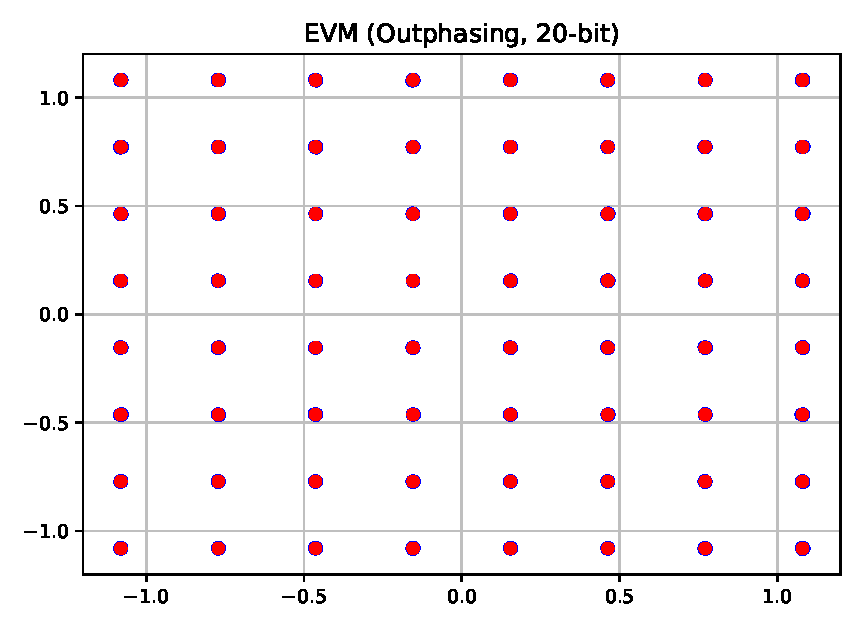
\includegraphics[width=0.48\textwidth]{Pics/evm_20bit_multop_v2.eps}
    \begin{itemize}
        \item EVM 0.34% 
    \end{itemize}
\end{frame}


%%%%%%%%%%%%%%%%%%%%%%%%%%%%%%%%%%%%%%%%%%
\renewcommand{\sectionname}{Hattrick: Outphasing transmitter}
\subsection*{\sectionname}
\begin{frame}[c]
    \frametitle{\sectionname}
    \begin{itemize}
        \item System verification
            \begin{itemize}
                \item  Replace the transmitter DSP with RTL models
                \item  Verify functionality
            \end{itemize}
    \end{itemize}
    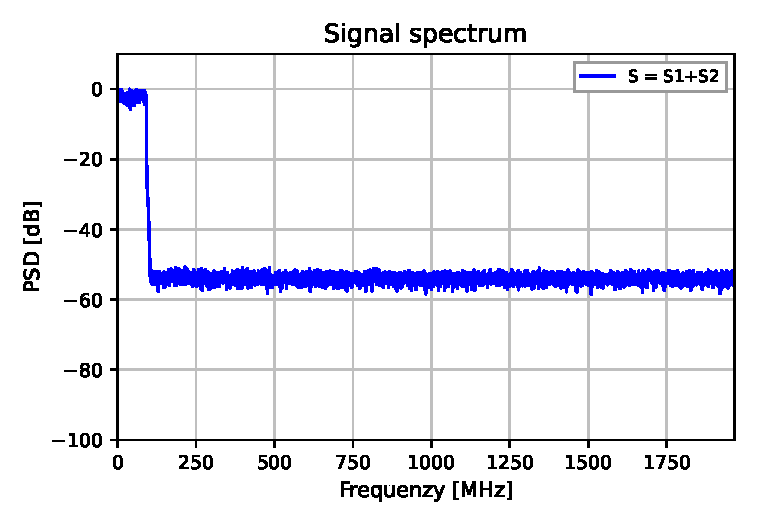
\includegraphics[width=0.48\textwidth]{Pics/scs_out1+2_10b_v2.eps}
    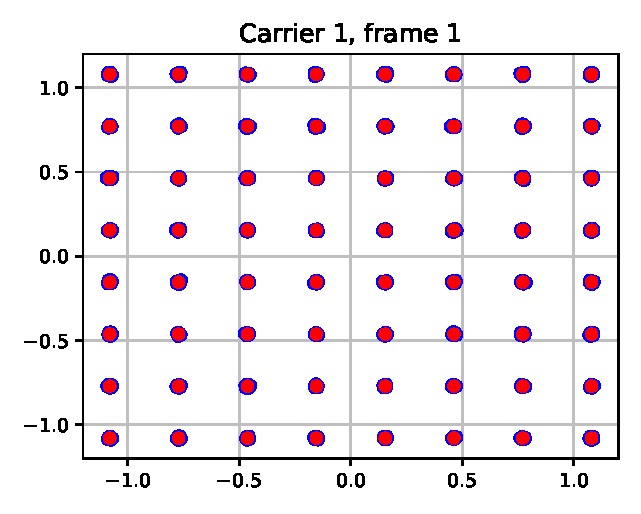
\includegraphics[width=0.48\textwidth]{Pics/evm_10bit_multop_v2.eps}
    \begin{itemize}
        \item EVM=0.60% 
    \end{itemize}
\end{frame}


%%%%%%%%%%%%%%%%%%%%%%%%%%%%%%%%%%%%%%%%%%%%%%%%%%%%%%%%%%%%%%%%%%%%%%%%%%%%%
\renewcommand{\sectname}{Conclusion}
\section{\sectname}
\begin{frame}[t]
    \frametitle{\sectname}
    \begin{itemize}
        \item Modular design environment through well defined IO boundaries and
            \emph{Entity} definitions.
        \item Open Source
        \item Automates repetitive verification tasks and provides means for programmatic
            verification with various simulators
        \item Support for measurement equipment under development.
        \item \emph{Enables} co-development by multiple designers using various
            verification tools.
        \item \emph{Enabled by} utilization of programming methodology and
            version control in hardware design context.
    \end{itemize}
\end{frame}


\end{document}
